\section{Reklama}
    \begin{quote}
        \enquote{\emph{Ačkoliv reklama je pouze jedna z částí komunikačního (propagačního) mixu, je to část, která je nejvíce vidět.
        Mezi hlavní cíle reklamy patří kromě zvýšení poptávky a vyvolání nové či opakované koupě především tvorba silné značky,
        která zaujímá pevné a přední místo v mysli zákazníka mající k ní pozitivní postoj, dále identifikace a
        odlišení produktu (značky) od podobných produktů nabízených na trhu,
        vytváření pozitivní image firmy nebo výrobku a budování tak preferencí a věrnosti, posílení finanční pozice podniku,
        zvýšení možnosti distribuce a snížení nákladů spojených s prodejem, ale i motivace vlastních pracovníků aj.}}
        (SVĚTLÍK, J., 2016) \cite{svetlik:marketing}
    \end{quote}
    

    Síla reklamy se skrývá i ve schopnosti ovlivňování názorů lidí. Tohoto si lze nejčastěji všimnout např.
    u politických stran. Nejčastější reklamy lze podle způsobu použití dělit na 2 kategorie. \cite{marketing:product-vs-brand}

    \subsection{Produktová reklama}
    Tento druh reklamy je zaměřený na nabízený produkt, který se snaží vyzdvihnout výhody nad konkurencí.
    Jde o konkrétní nabízené služby nebo výrobky. Vhodné využití této reklamy je následující:
    \begin{itemize}
        \item Pokud je potřeba produktem oslovit velké publikum.
        \item Pokud je produkt skutečně \enquote{něčím dosud neviděným}.
        \item Pokud produkt \enquote{dokáže mluvit za sebe}.
    \end{itemize}

    \subsection{Značková reklama}
    Oproti produktové reklamě, se zde jedná spíše o zaujetí zákazníka jako takového. Nenabízí žádný konkrétní produkt,
    snaží se dostat zákazníkovi do podvědomí. Je výhodná pokud:
    \begin{itemize}
        \item Si značka chce vybudovat unikátní postavení na trhu. 
        \item Značka má zajímavý příběh o vzniku nebo historické pozadí. 
        \item Je prioritou budovat si zákaznickou důvěru značce. 
    \end{itemize}

    \subsection{Reklamní média}
    Jak tato práce výše zmiňuje, volba reklamního média závisí na cílové skupině, kterou se snaží oslovit.
    Správná volba dokáže pozitivně ovlivnit účinnost reklamy, zatímco špatný výběr může přinést pouze finanční zátěž.
    Média nejčastěji doručují význam reklamního sdělení 3 způsoby:
    \begin{enumerate}
        \item verbálně,
        \item zvukově,
        \item obrazově.
    \end{enumerate}
    Tato část práce rozebírá nejpoužívanější reklamní nosiče a jejich výhody. \cite{typy:medii} \cite{typy:mediatypy}
    
    \subsubsection{Tisk}
    Do této skupiny patří zejména periodické publikace jako noviny a časopisy. Tiskoviny jako katalogy, ročenky a zpravodaje zde lze také zařadit.
    Výhody tisku spočívají v geografickém zaměření -- možnost celostátního zaměření nebo jen jednotlivých regionů. Komerční sdělení se dá umístit k tématicky
    vhodným sekcím nebo časopisům. Zákazník při čtení novin a časopisů stráví více času na rozdíl od televize nebo rozhlasu,
    a proto mohou být sdělení obsáhlejší a komplexnější. Poslední výhodou jsou \emph{packshoty}, neboli společné balení inzerovaného produktu s magazínem.
    
    \subsubsection{Rozhlas}
    Rádia stejně jako noviny je možno použít pro možnost zaměření, a to nejen zeměpisným ale také časovým. Často se však stává,
    že se z rádia stane pouze kulisa na pozadí a člověk jej nevnímá. Působí pouze na jeden lidský smysl -– sluch,
    což pro nabízení určitých služeb či produktů nemusí stačit.

    \subsubsection{Outdoor}
    K této skupině se řadí jako nejpoužívanější média billboardy, citylighty, bigboardy, LED plochy a ostatní venkovní velké plochy nebo nápisy včetně
    firemních štítů, plakátů, MHD atd. Tyto nosiče setrvávají na svých místech a působí na lidi dlouhodobě, občas i vícekrát za den.
    Dají se zaměřovat od celostátního působení až na malá místa jako části měst. Nevýhodou je, že velice závisí na své lokalitě, viditelnosti a
    nemohou obsahovat složitá sdělení. 

    \subsubsection{Televize}
    Audiovizuální prezentace přes televize je jeden z nejúčinnějších prostředků komunikací s možným koncovým zákazníkem.
    Má široký rozsah uživatelů, dokáže nejlépe vyvolat emoce a asociace se značkou. Reklama se dá lépe cílit na základě měření sledovanosti.
    Její cena je však vysoká a je zde možnost, že si uživatel televize přepne kanál, aby nemusel reklamu sledovat.
    Navíc televizní inzerce se musí plánovat s předstihem z důvodů nepružných vysílacích plánů.
    
    \subsubsection{Kino}
    Ačkoli se tento typ média zdá nenápadným, má vysokou sledovanost. Divák je pohodlně usazen a v očekávání filmu věnuje svou pozornost všemu na promítacím plátně před sebou.
    Navíc je vše v perfektní kvalitě, jak zvukové, tak vizuální. Důležitým aspektem je vybrat kina s vysokou návštěvností a naplánovat reklamní kampaň předem, ideálně vložit spoty před promítání úspěšných projekcí.

    \subsubsection{Online}
    Internet je nejflexibilnější reklamní médium. Využívá jej velká část populace a rychle se rozrůstá. Nabízí různé možnosti inzercí, formátů,
    vysokou přesnost zaměření a jednoduchý monitoring. Jako jediný z výše zmíněných umožňuje interaktivní reklamu. Nabízí dobrou kontrolu nákladů a konverzí.
    Tři nejčastější způsoby platby jsou:
    \begin{itemize}
        \item PPV -- platba za zobrazení.
        \item PPA -- platba za nějakou akci (přihlášení k newsletteru, prodej, \ldots).
        \item PPC -- platba za proklik.
    \end{itemize}
    Internet přitáhl spoustu inzerentů a každý chce být co nejvíce viděn. Tímto vznikla vysoká konkurence mezi inzerenty, kdo zaplatí nejvíce za zobrazení své reklamy.
    Velký počet reklam na webu zase zapříčinil, že běžní uživatelé se chtějí reklamě vyhnout a snaží se jí blokovat.
    
    \subsubsection{Srovnání reklamních médií}
    Průzkum inzertních výkonů SPIR 2020 odhaluje, že i přes velké možnosti Internetu, je v České republice stále nejvíce investováno do reklamy televizní.
    Celkové srovnání medií se nachází na obrázku \ref{fig:spir-mediatypes}.


    \begin{figure}[h]
        \centering
        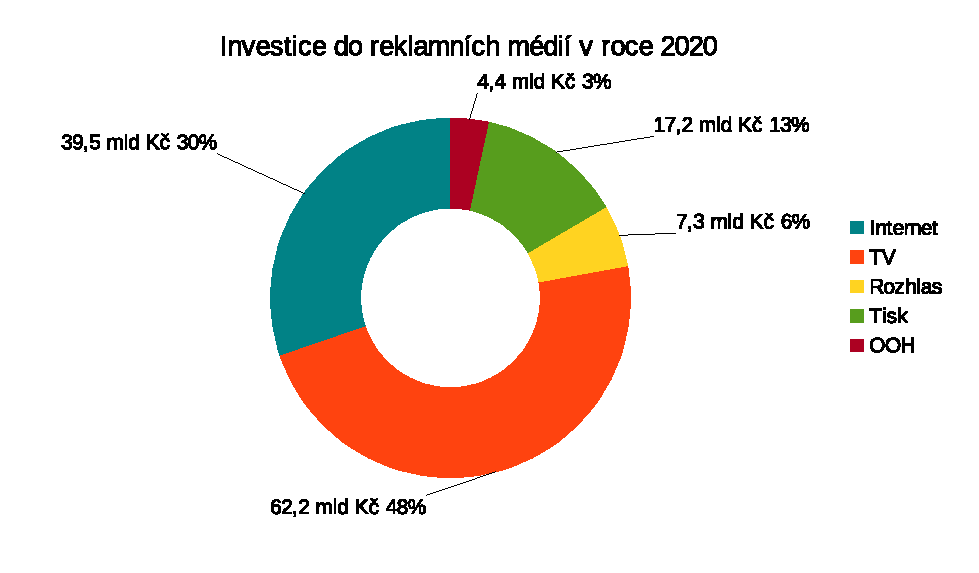
\includegraphics[width=0.9\textwidth]{Figures/pie-chart.eps}
        \iffalse
        This is my multi-line comment
        % \includesvg{Figures/pie-chart}
        % \begin{tikzpicture}
        %     \pie[
        %         text=pin,
        %         after number=~mld.,
        %         sum=auto,
        %     ]{39.5/Internet,
        %     62.2/TV,
        %     4.4/OOH,
        %     17.2/Tisk,
        %     7.3/Rozhlas}
        % \end{tikzpicture}
        \fi

        \caption[Podíl mediatypů v roce 2020]{Podíl jednotlivých mediatypů v roce 2020 \cite{spir:mediatypes}}
        \label{fig:spir-mediatypes}
    \end{figure}

    Možnosti online reklamy jsou velice rozsáhlé a stále se vyvíjejí. Následující kapitola se více zaměřuje na možnosti Internetové inzerce.